\documentclass[12pt]{article}
\usepackage[letterpaper, margin=1in]{geometry}
\usepackage{graphicx}
\graphicspath{{./Figures/}}
\usepackage{hyperref}
\usepackage{parskip}
\usepackage{amsmath}
\usepackage[framed, numbered]{matlab-prettifier}
\lstset{inputpath=../MATLAB}

\DeclareMathOperator{\sinc}{sinc}
\DeclareMathOperator{\rect}{rect}

\title{ELECENG 3TR4 Lab 2: Amplitude Modulation}
\author{
    Aaron Pinto \\ pintoa9
    \and
    Raeed Hassan \\ hassam41
}

\begin{document}

\maketitle
\clearpage

% don't have to do sections, can probably just do a numbered list but this might look nicer
\section*{Message Signal}
The message signal is given by Equation~\ref{eq:message_signal}. In the equation, $T_m = 0.0005$ s.
\begin{equation} \label{eq:message_signal}
    m(t) = -2\sinc(t/T_m)
\end{equation}
The message signal is plotted in the time and frequency domain in Figure~\ref{fig:message_signal}. The frequency domain plot features the magnitude spectrum of the message signal. The MATLAB code used to generate the message signal and its plots are in the lab2.m MATLAB script. A portion of the MATLAB code used to generate and plot the message signal is shown in Listing~\ref{listing:message_signal}.
\lstinputlisting[style=Matlab-editor, caption={Generating the Message Signal and Message Signal Plots}, label={listing:message_signal}, firstline=23, firstnumber=23, lastline=55]{lab2.m} 
\begin{figure}[h!]
    \centering
    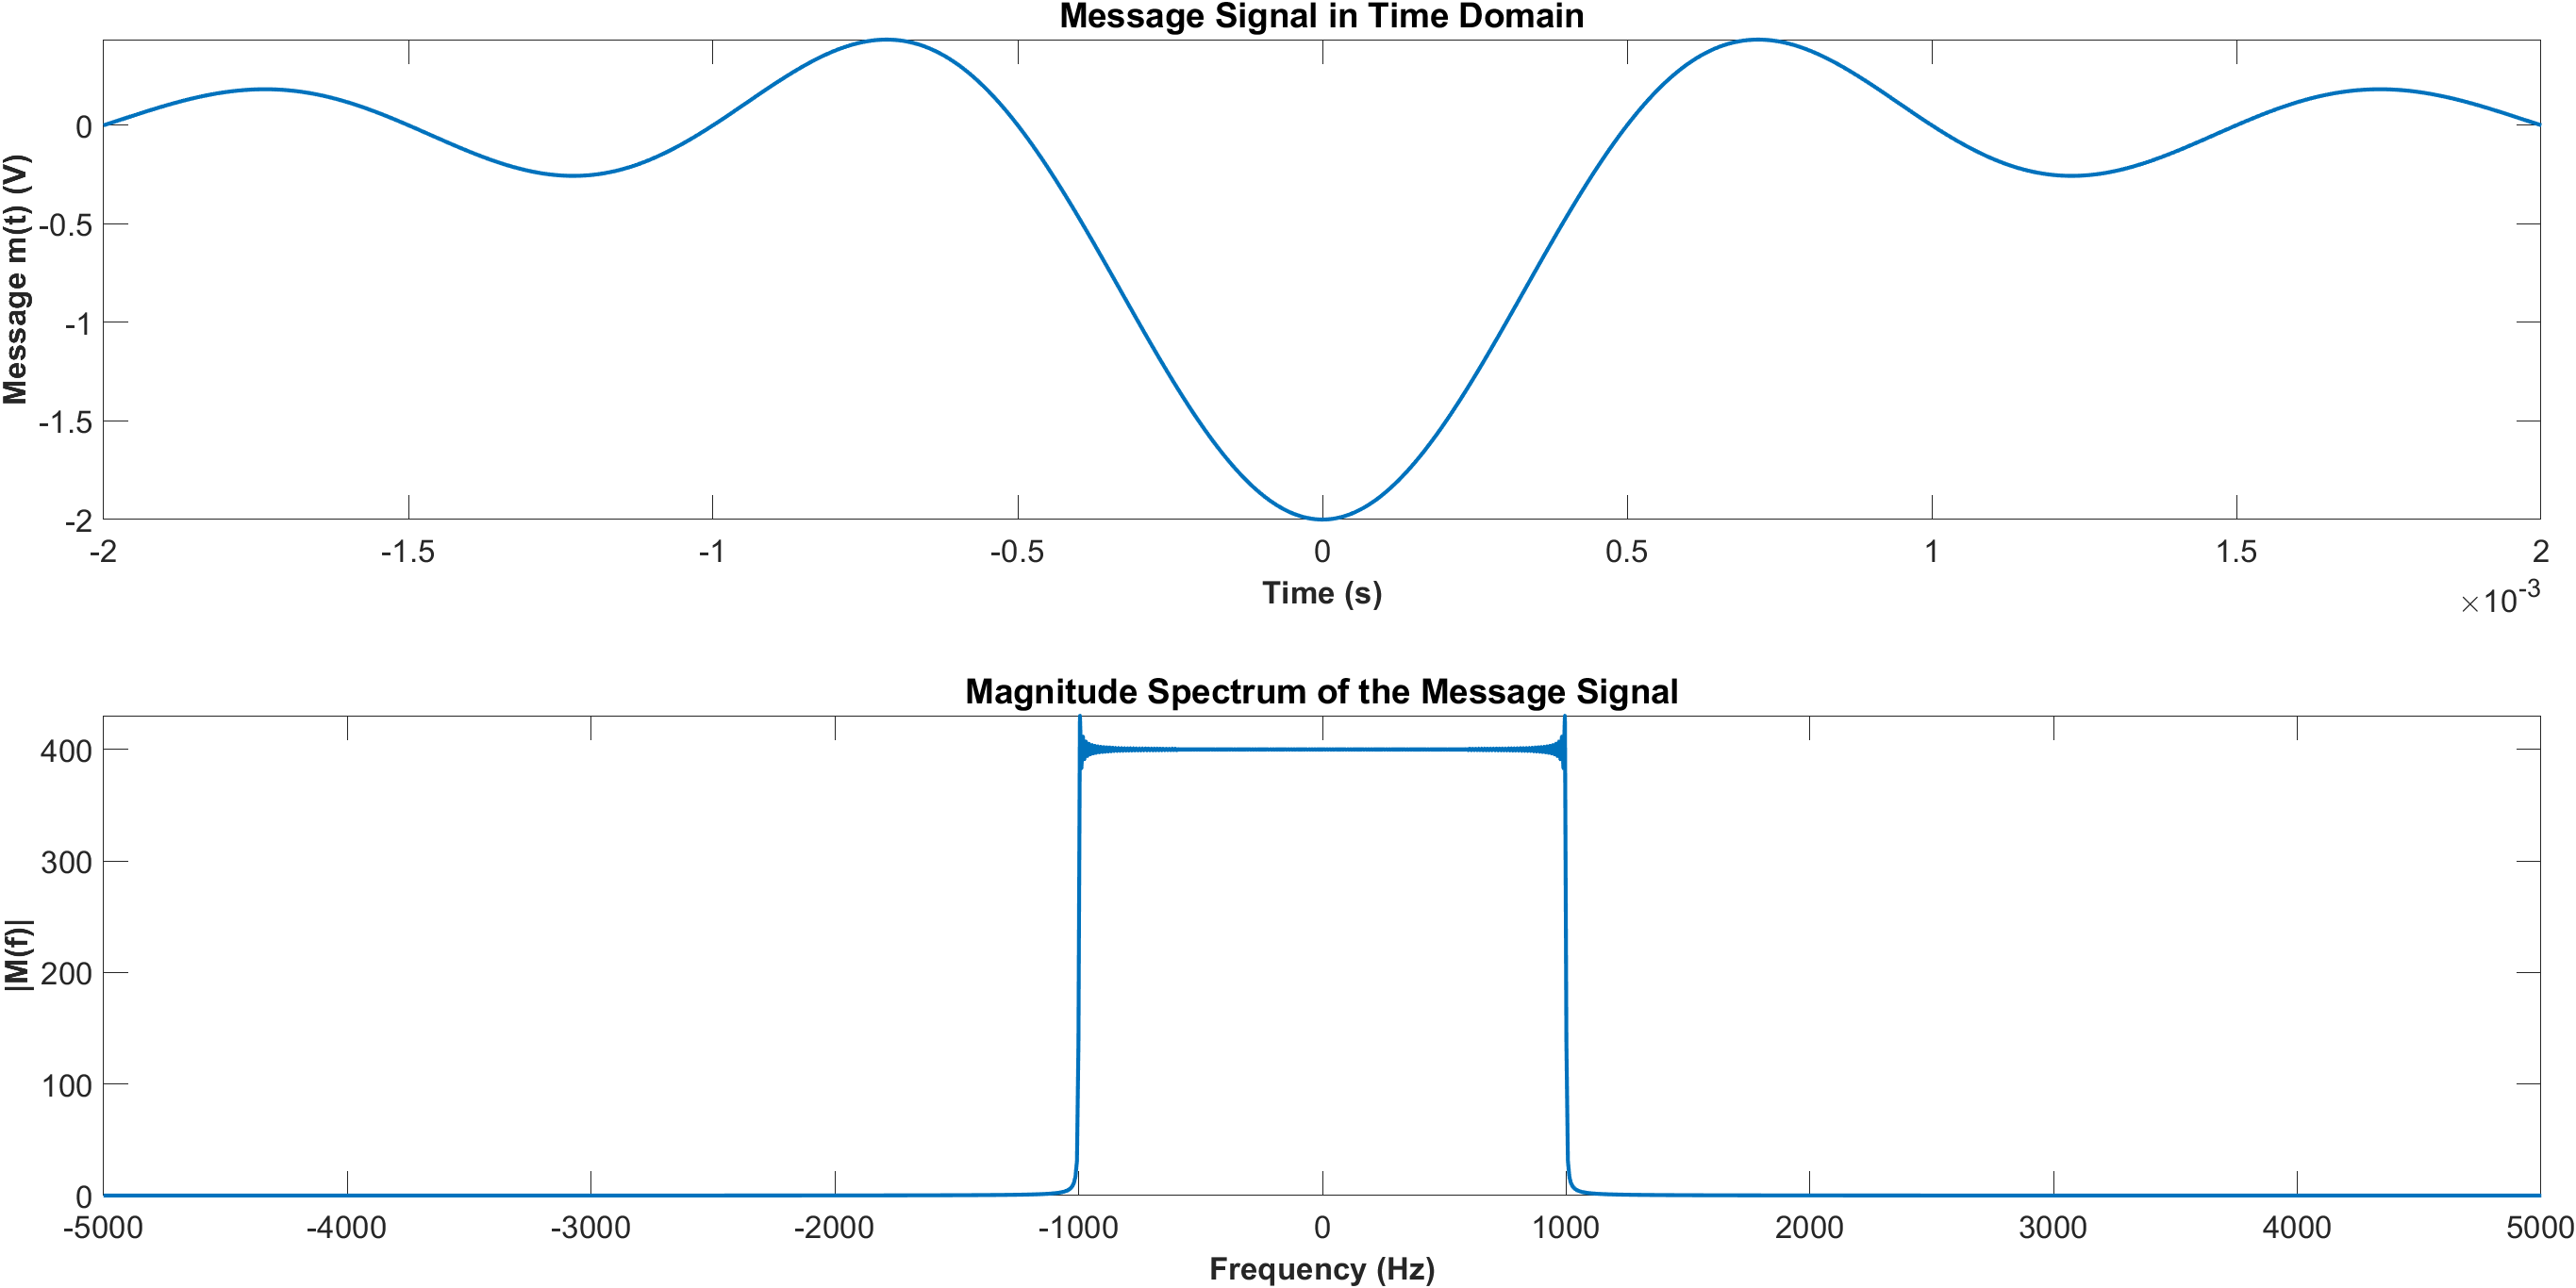
\includegraphics[width=\textwidth]{q1}
    \caption{\label{fig:message_signal}Message Signal Plots}
\end{figure}
The highest frequency component of the signal occurs at 995 Hz, which is the frequency bin that is closest to 1000 Hz. An analytical calculation of the magnitude spectrum of the message signal is done in Equation~\ref{eq:message_calc}. When $T_m = 0.0005$, the rect function representing the magnitude spectrum of the message signal ranges from $-1000$ to $1000$, which matches the magnitude spectrum we plotted in MATLAB.
\begin{equation} \label{eq:message_calc}
\begin{aligned}[b]
    m(t) &\rightleftharpoons M(f) \\
    -2\sinc(t/T_m) &\rightleftharpoons M(f) \\
    \sinc(t) &\rightleftharpoons \rect(f) \\
    \sinc\left(\frac{1}{T_m} t\right) &\rightleftharpoons \left|T_m\right|\rect(T_m f) \\
    -2\sinc(t/T_m) &\rightleftharpoons -2\left|T_m\right|\rect(T_m f) \\
    M(f) &= -2\left|T_m\right|\rect(T_m f)
\end{aligned}
\end{equation}

\section*{Amplitude Modulation}
The modulated signal is given by Equation~\ref{eq:am_signal}. The carrier is given by the $c(t) = A_c \cos(2\pi f_c t)$ where $A_c = 1$ V and $f_c = 20$ kHz. 
\begin{equation} \label{eq:am_signal}
    s(t) = A_c \left[ 1 + k_a m(t) \right] \cos(2\pi f_c t)
\end{equation}
The MATLAB code used to generate the modulated signal is shown in Listing~\ref{listing:mod_50_signal}. The MATLAB function modulated\_fig that is used to generate the plots for the modulated signal is shown in Listing~\ref{listing:mod_plot}.
\lstinputlisting[style=Matlab-editor, caption={Generating the Modulated Signal}, label={listing:mod_50_signal}, firstline=66, firstnumber=66, lastline=72]{lab2.m}
\lstinputlisting[style=Matlab-editor, caption={Generating the Modulated Signal Plots}, label={listing:mod_plot}, firstline=130, firstnumber=130, lastline=159]{lab2.m}
The modulated signal with 50\% modulation is plotted in the time and frequency domain in Figure~\ref{fig:am_signal}. The frequency domain plot features the magnitude spectrum of the modulated signal.
\begin{figure}[h!]
    \centering
    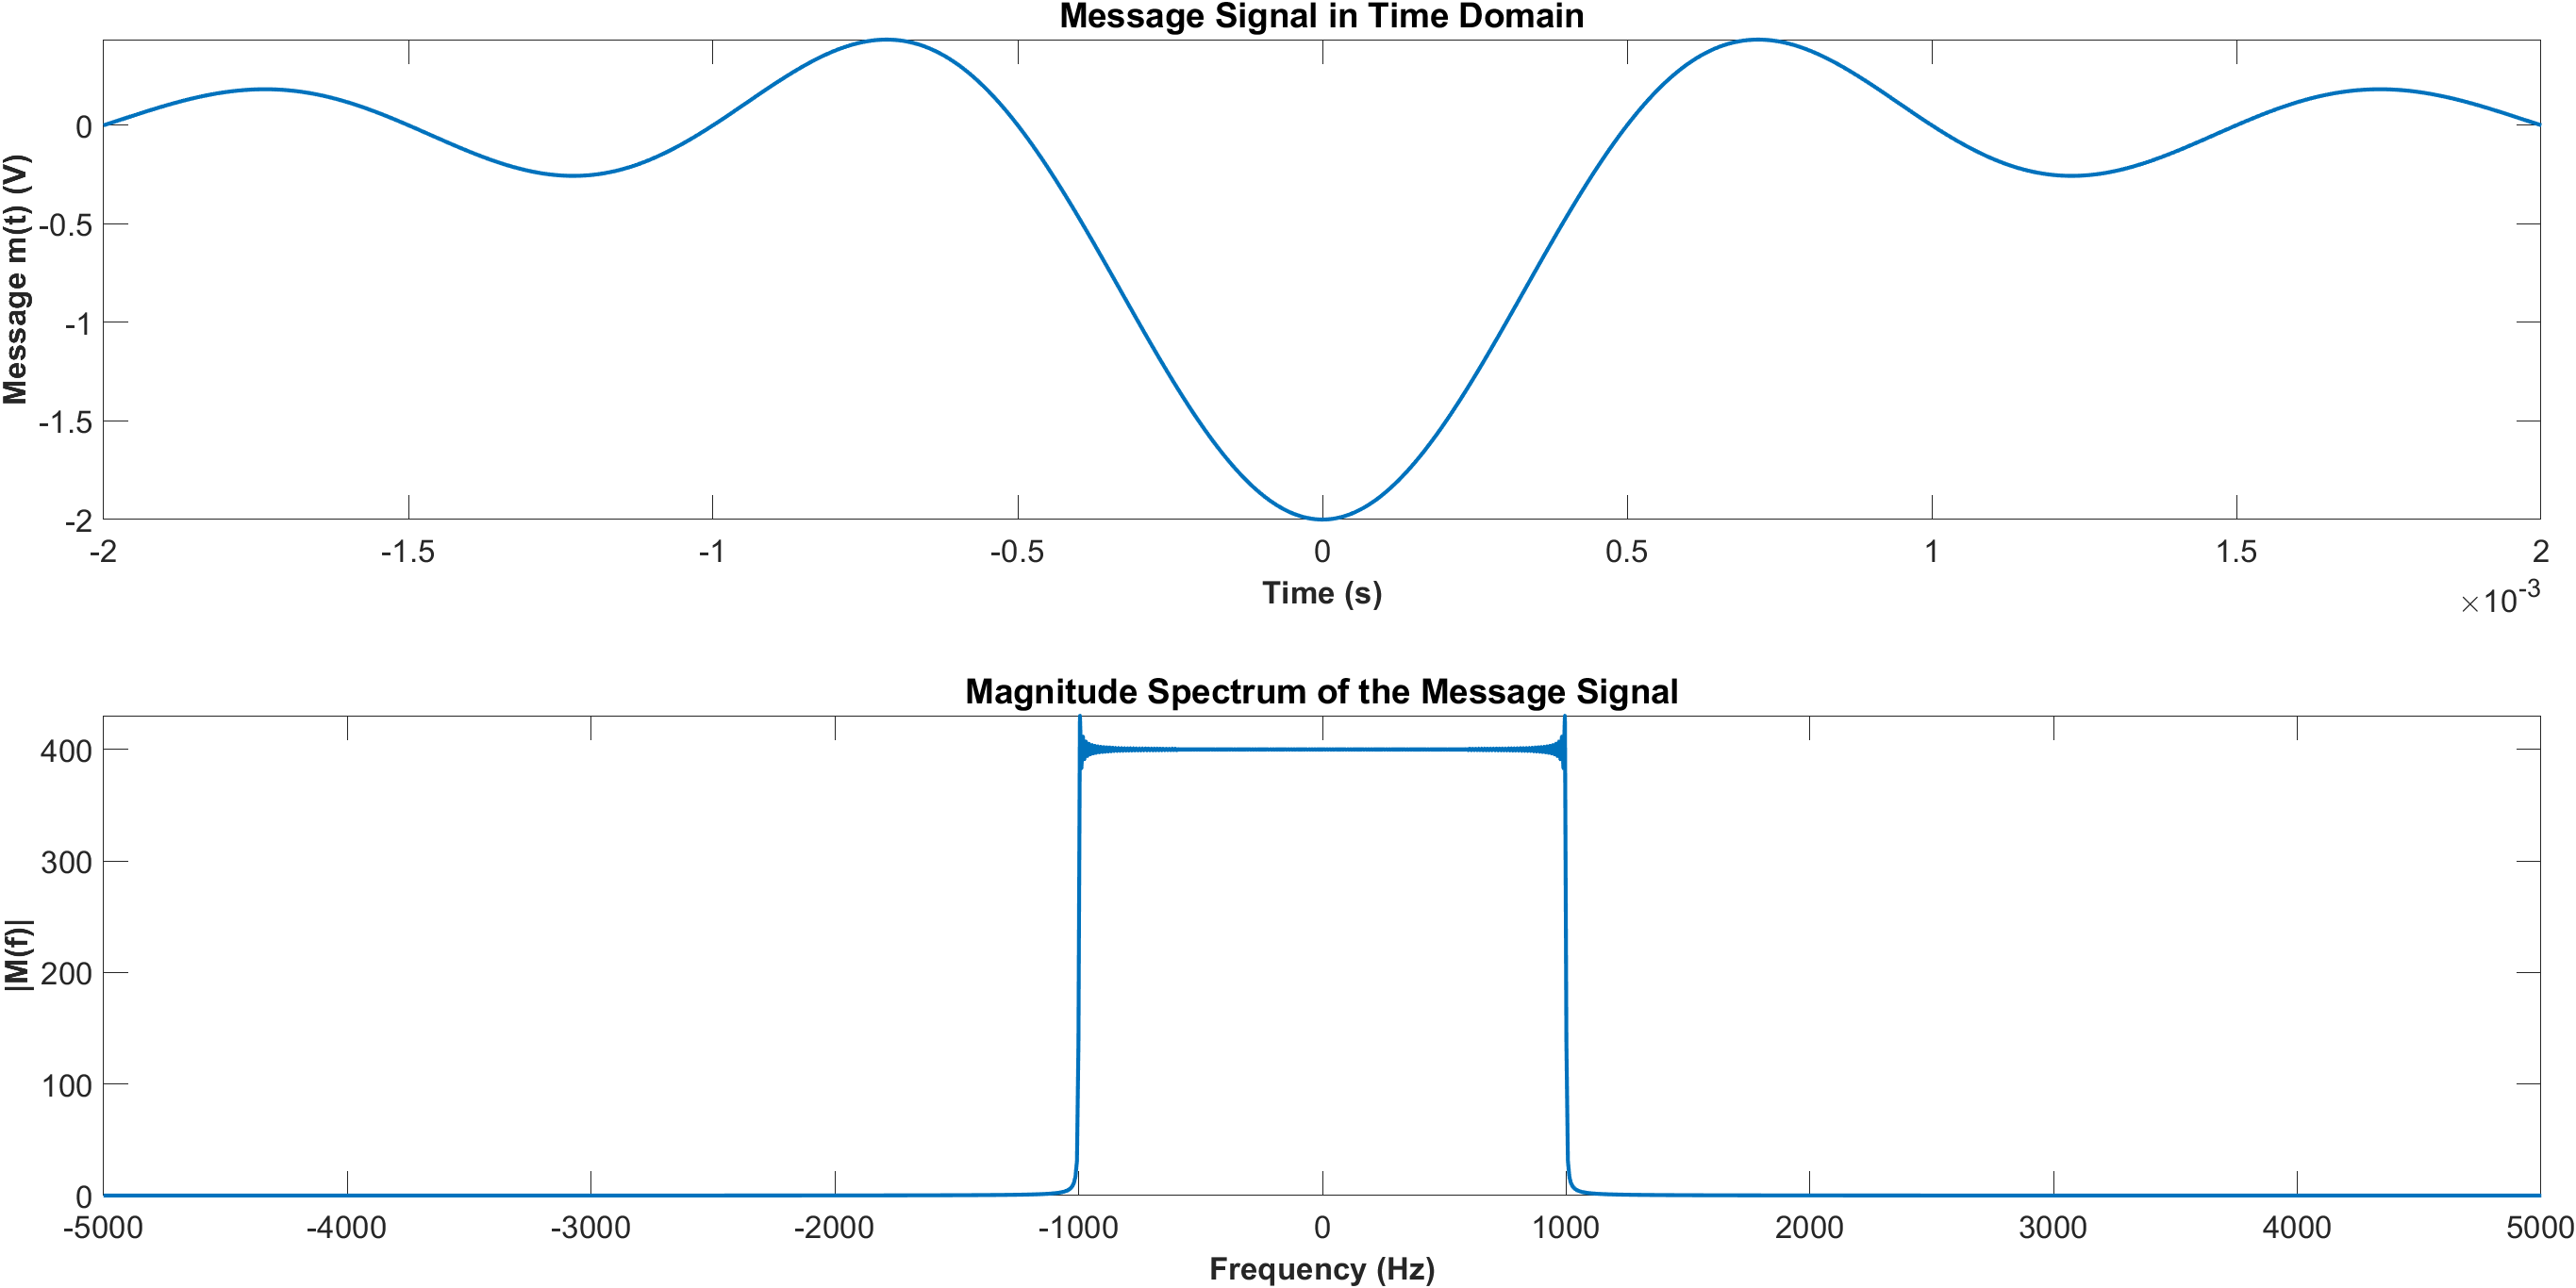
\includegraphics[width=\textwidth]{q2}
    \caption{\label{fig:am_signal}Modulated Signal with 50\% Modulation}
\end{figure}

\section*{Amplitude Demodulation}
To demodulate the signal, we pass the modulated signal through an envelope detector and then remove the DC component of the signal. The MATLAB function envelope\_detector to pass the signal through an envelope detector is shown in Listing~\ref{listing:envelope}. The MATLAB function output\_fig is to plot the demodulated plots, and a snippet of it is shown in Listing~\ref{listing:demod}.
\lstinputlisting[style=Matlab-editor, caption={Envelope Detector}, label={listing:envelope}, firstline=166, firstnumber=166, lastline=189]{lab2.m}
\lstinputlisting[style=Matlab-editor, caption={Demodulating the Signal}, label={listing:demod}, firstline=205, firstnumber=205, lastline=226]{lab2.m}

\subsection*{Output Signals for Time Constant $R_LC = 1/f_c$}
The output signals after demodulation for when the time constant of the envelope detector is set to $R_LC = 1/f_c$ are shown in Figure~\ref{fig:q2i}. We can observe that the upper envelope of the output signal does follow the original message signal closely, but there is significant rippling in the output signal. The rippling in the signal would introduce a significant offset if the signal is passed through a low-pass filter to reduce the rippling, as we can see that the center of the rippled message is significantly below the upper envelope of the output signal. The significant rippling suggests that the time constant used in this scenario is too low.
\begin{figure}[h!]
    \centering
    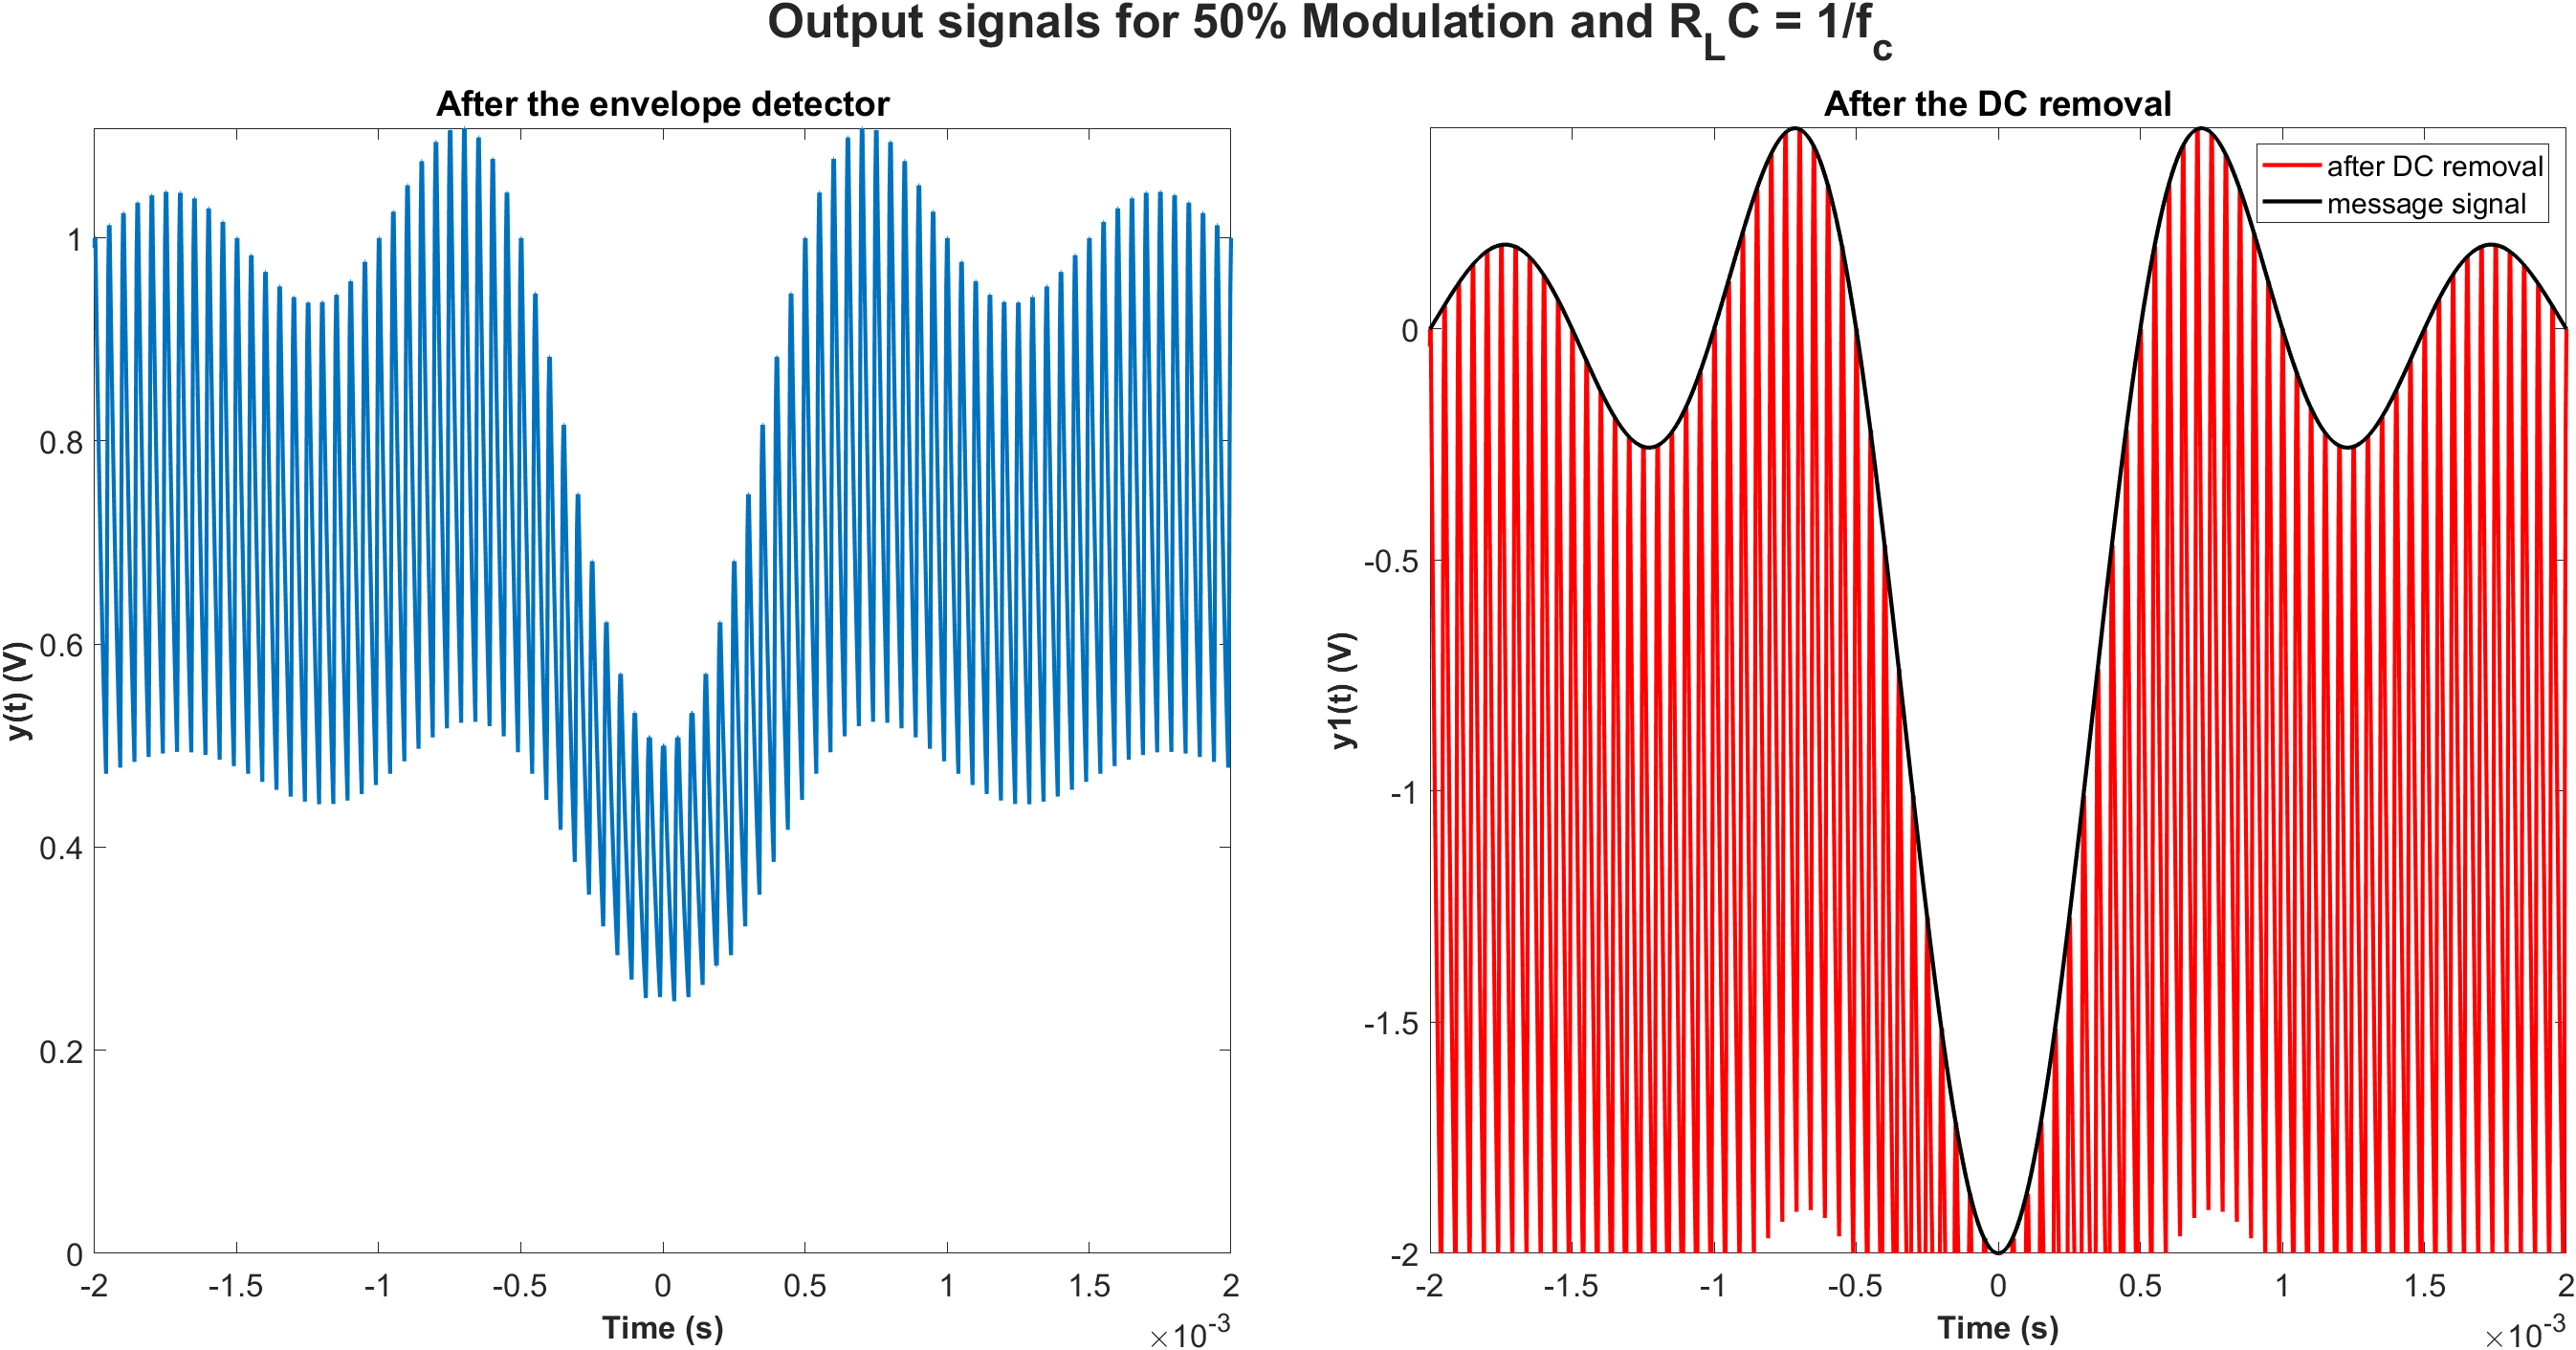
\includegraphics[width=\textwidth]{q2i}
    \caption{\label{fig:q2i}Demodulation Output for $R_LC = 1/f_c$}
\end{figure}

\subsection*{Output Signals for Time Constant $R_LC = 10T_m$}
The output signals after demodulation for when the time constant of the envelope detector is set to $R_LC = 10T_m$ are shown in Figure~\ref{fig:q2ii}. We can observe that the output signal lags behind the input signal significantly whenever there is a drop in the input signal, and the curve following the increasing portions of the input signal is very jagged. A significant portion of the input signal is lost whenever the is a drop in the input signal, and it would be impossible to accurately retrieve the input signal whenever the signal decreases too rapidly for the envelope to follow. The significant delay in following the input signal suggests that the time constant used in this scenario is too high.
\begin{figure}[h!]
    \centering
    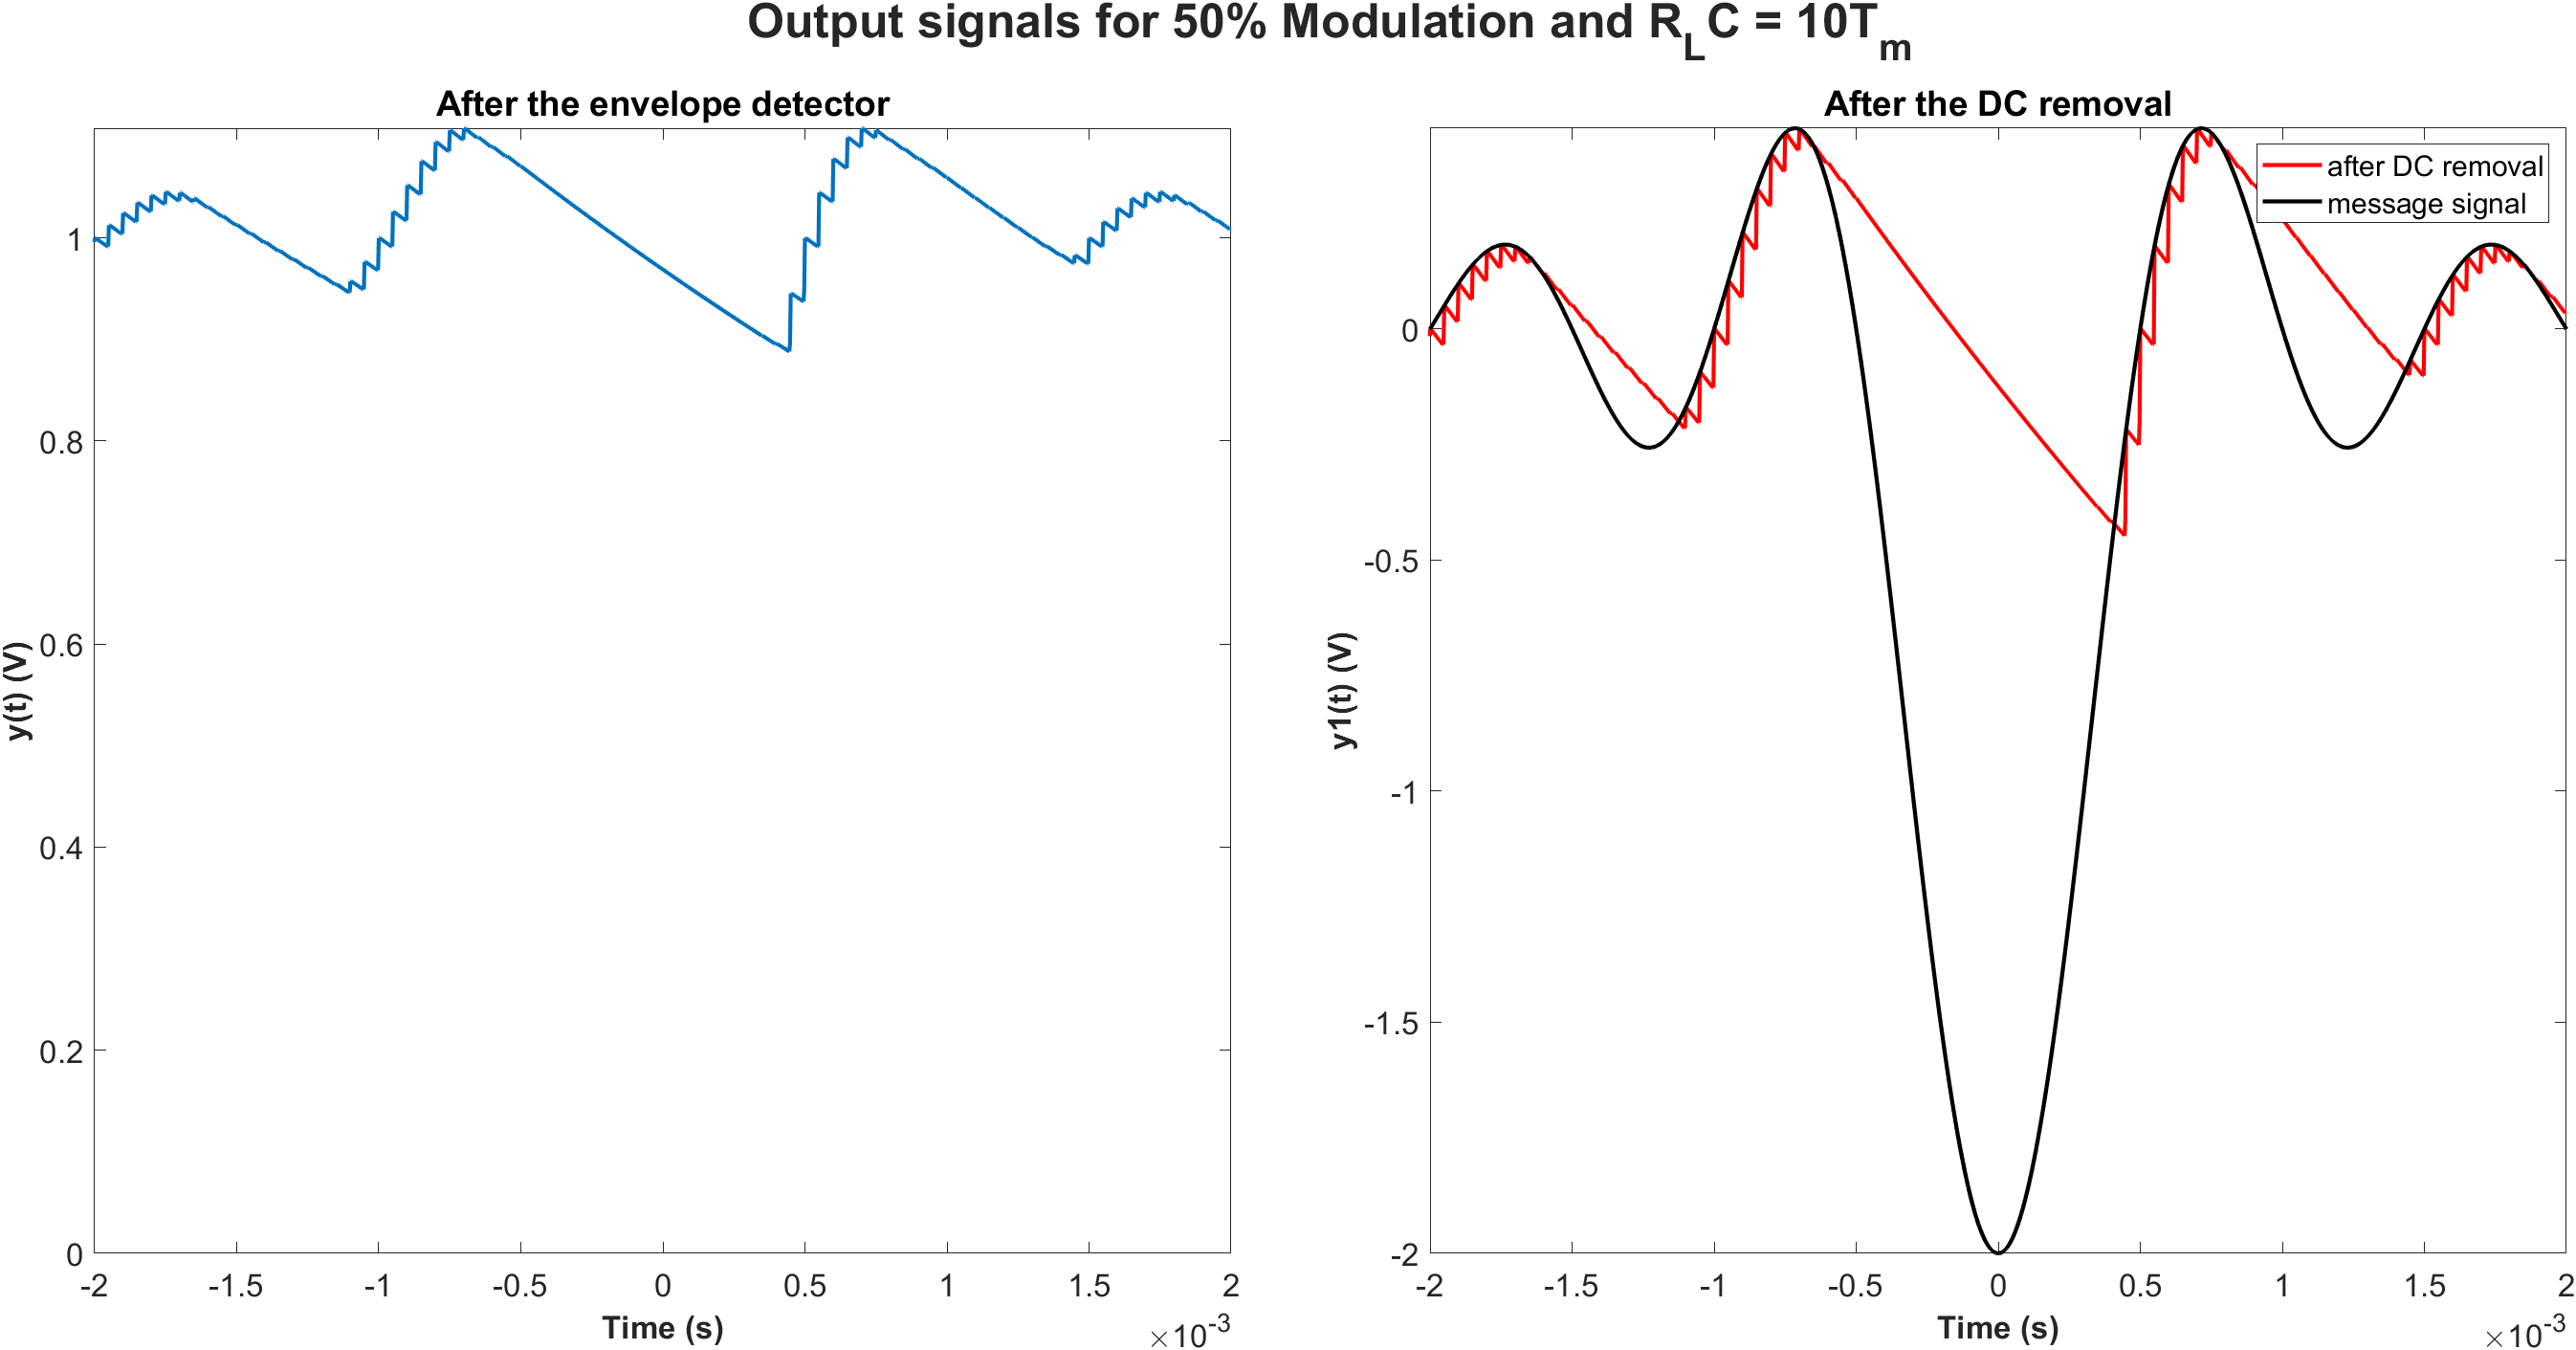
\includegraphics[width=\textwidth]{q2ii}
    \caption{\label{fig:q2ii}Demodulation Output for $R_LC = 10T_m$}
\end{figure}

\subsection*{Determining the Optimal Time Constant}
%1.1T_m = T_m + 1/f_c.
Based on the observations of the output signal for when the time constant is equal to $R_LC = 1/f_c$ and $R_LC = 10T_m$, we can conclude that the optimal range of time constants for the envelope likely falls between the two values. We started with a time constant of $T_m$, which falls in the middle of the two values and found that it had followed the signal relatively well without having excessive rippling. As we explored values around $T_m$, we concluded that $R_LC = 1.1T_m = T_m + 1/f_c$ was the optimal value for the time constant that minimized rippling while still closely following the input signal. Time constant values from around $0.7T_m$ to $1.25T_m$ also did not differ very much from $R_LC = T_m + 1/f_c$, and could be considered to be adequate. We also passed this output signal through a low-pass filter after DC removal, using a filter generated through the built-in MATLAB function lowpass. The low-pass filter are shown in Figure~\ref{fig:lpf}. The output signals after demodulation for when the time constant of the envelope detector is set to $R_LC = T_m + 1/f_c$ are shown in Figure~\ref{fig:q2iii}.
\begin{figure}[h!]
    \centering
    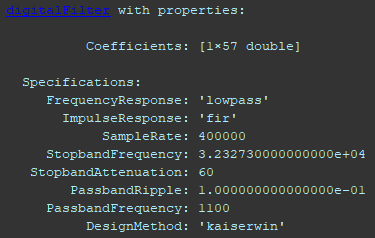
\includegraphics[width=0.57\textwidth]{lpf}
    \caption{\label{fig:lpf}LPF Specifications}
\end{figure}
\begin{figure}[h!]
    \centering
    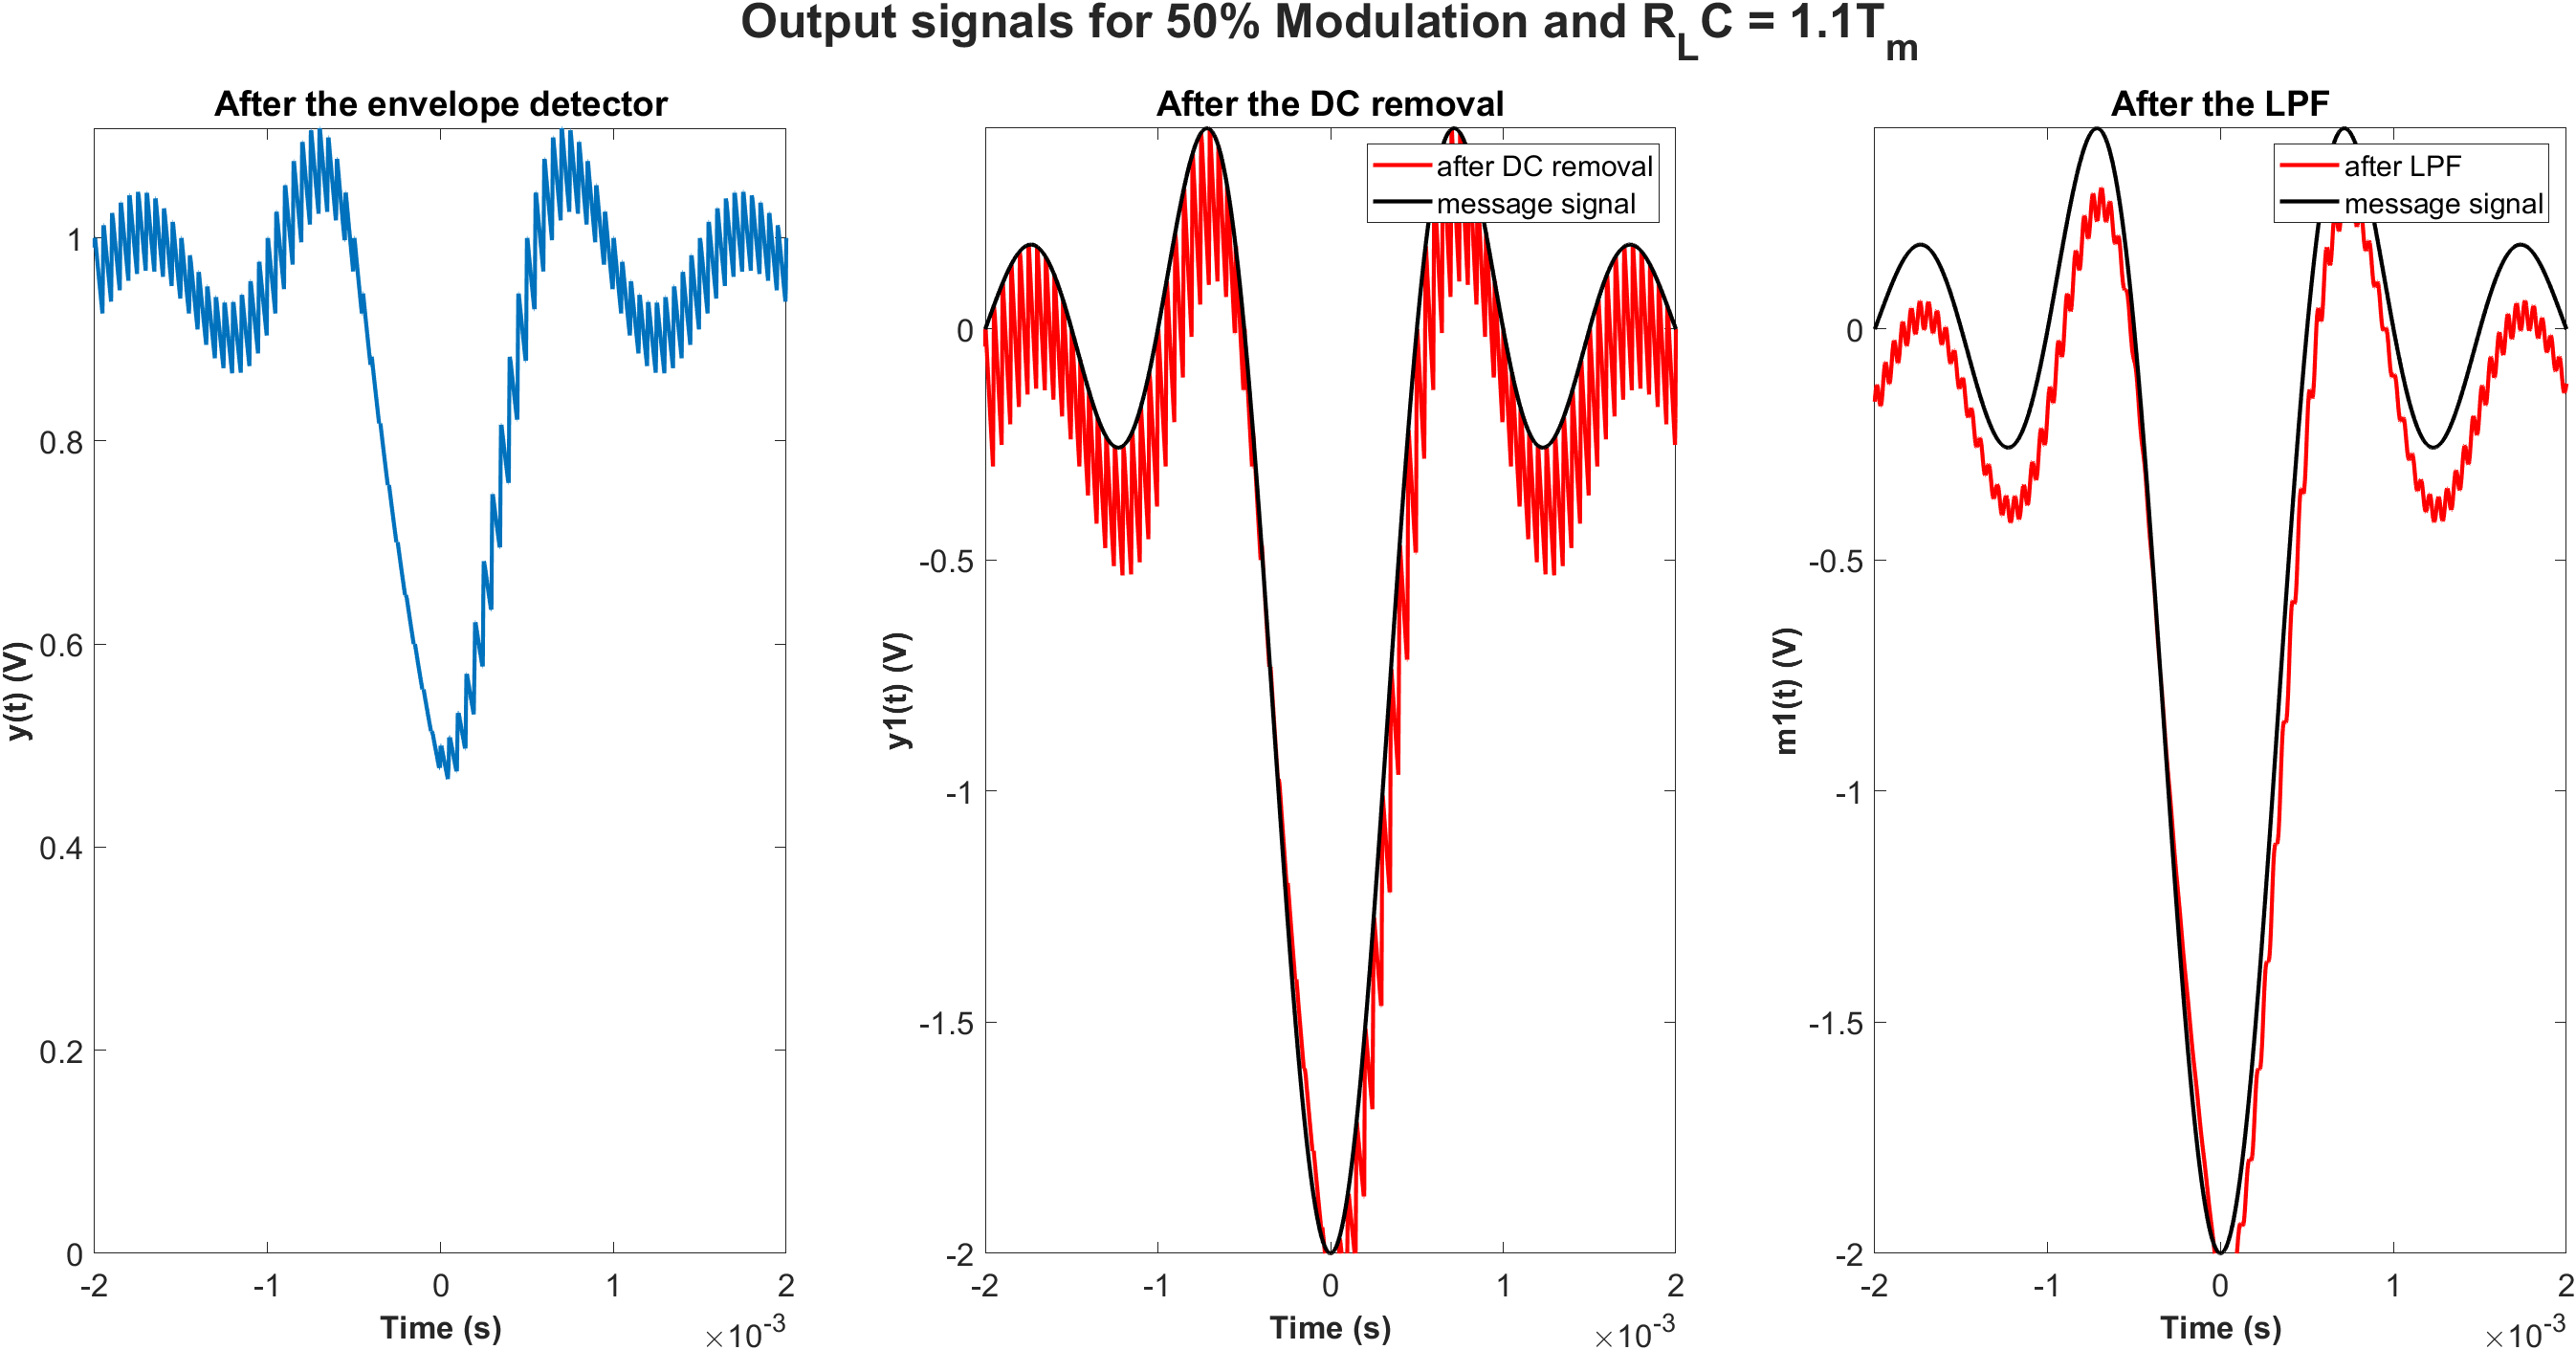
\includegraphics[width=\textwidth]{q2iii}
    \caption{\label{fig:q2iii}Demodulation Output for $R_LC = 1.1T_m$}
\end{figure}

\section*{Amplitude Modulation with over 100\% Modulation}
The envelope detector can only detect the positive (upper) envelope of the signal. Therefore, whenever the envelopes of the signal change signs, the envelope detector is unable to retrieve the desired input signal. This can be seen when the same message signal and carrier are modulated with 200\% modulation instead of 50\% modulation. The modulated signal with 200\% modulation is shown in Figure~\ref{fig:q3_mod}. We can observe that the envelope of the signal (in dashed red lines) cross the y-axis multiple times, where the modulated signal in blue will also flip signs. The envelope detector will be able to realize that the sign of the envelope has changed, and will simply follow the upper envelope in those regions. Figure~\ref{fig:q3_demod} shows the demodulated sign after envelope detection, DC removal, and low-pass filtering. We can observe that the region of the demodulated signal where the modulated signal envelope flipped signs does not match the message signal. Therefore, we can conclude that it is impossible to retrieve a signal through amplitude modulation and demodulation when there is over 100\% modulation.
\begin{figure}[h!]
    \centering
    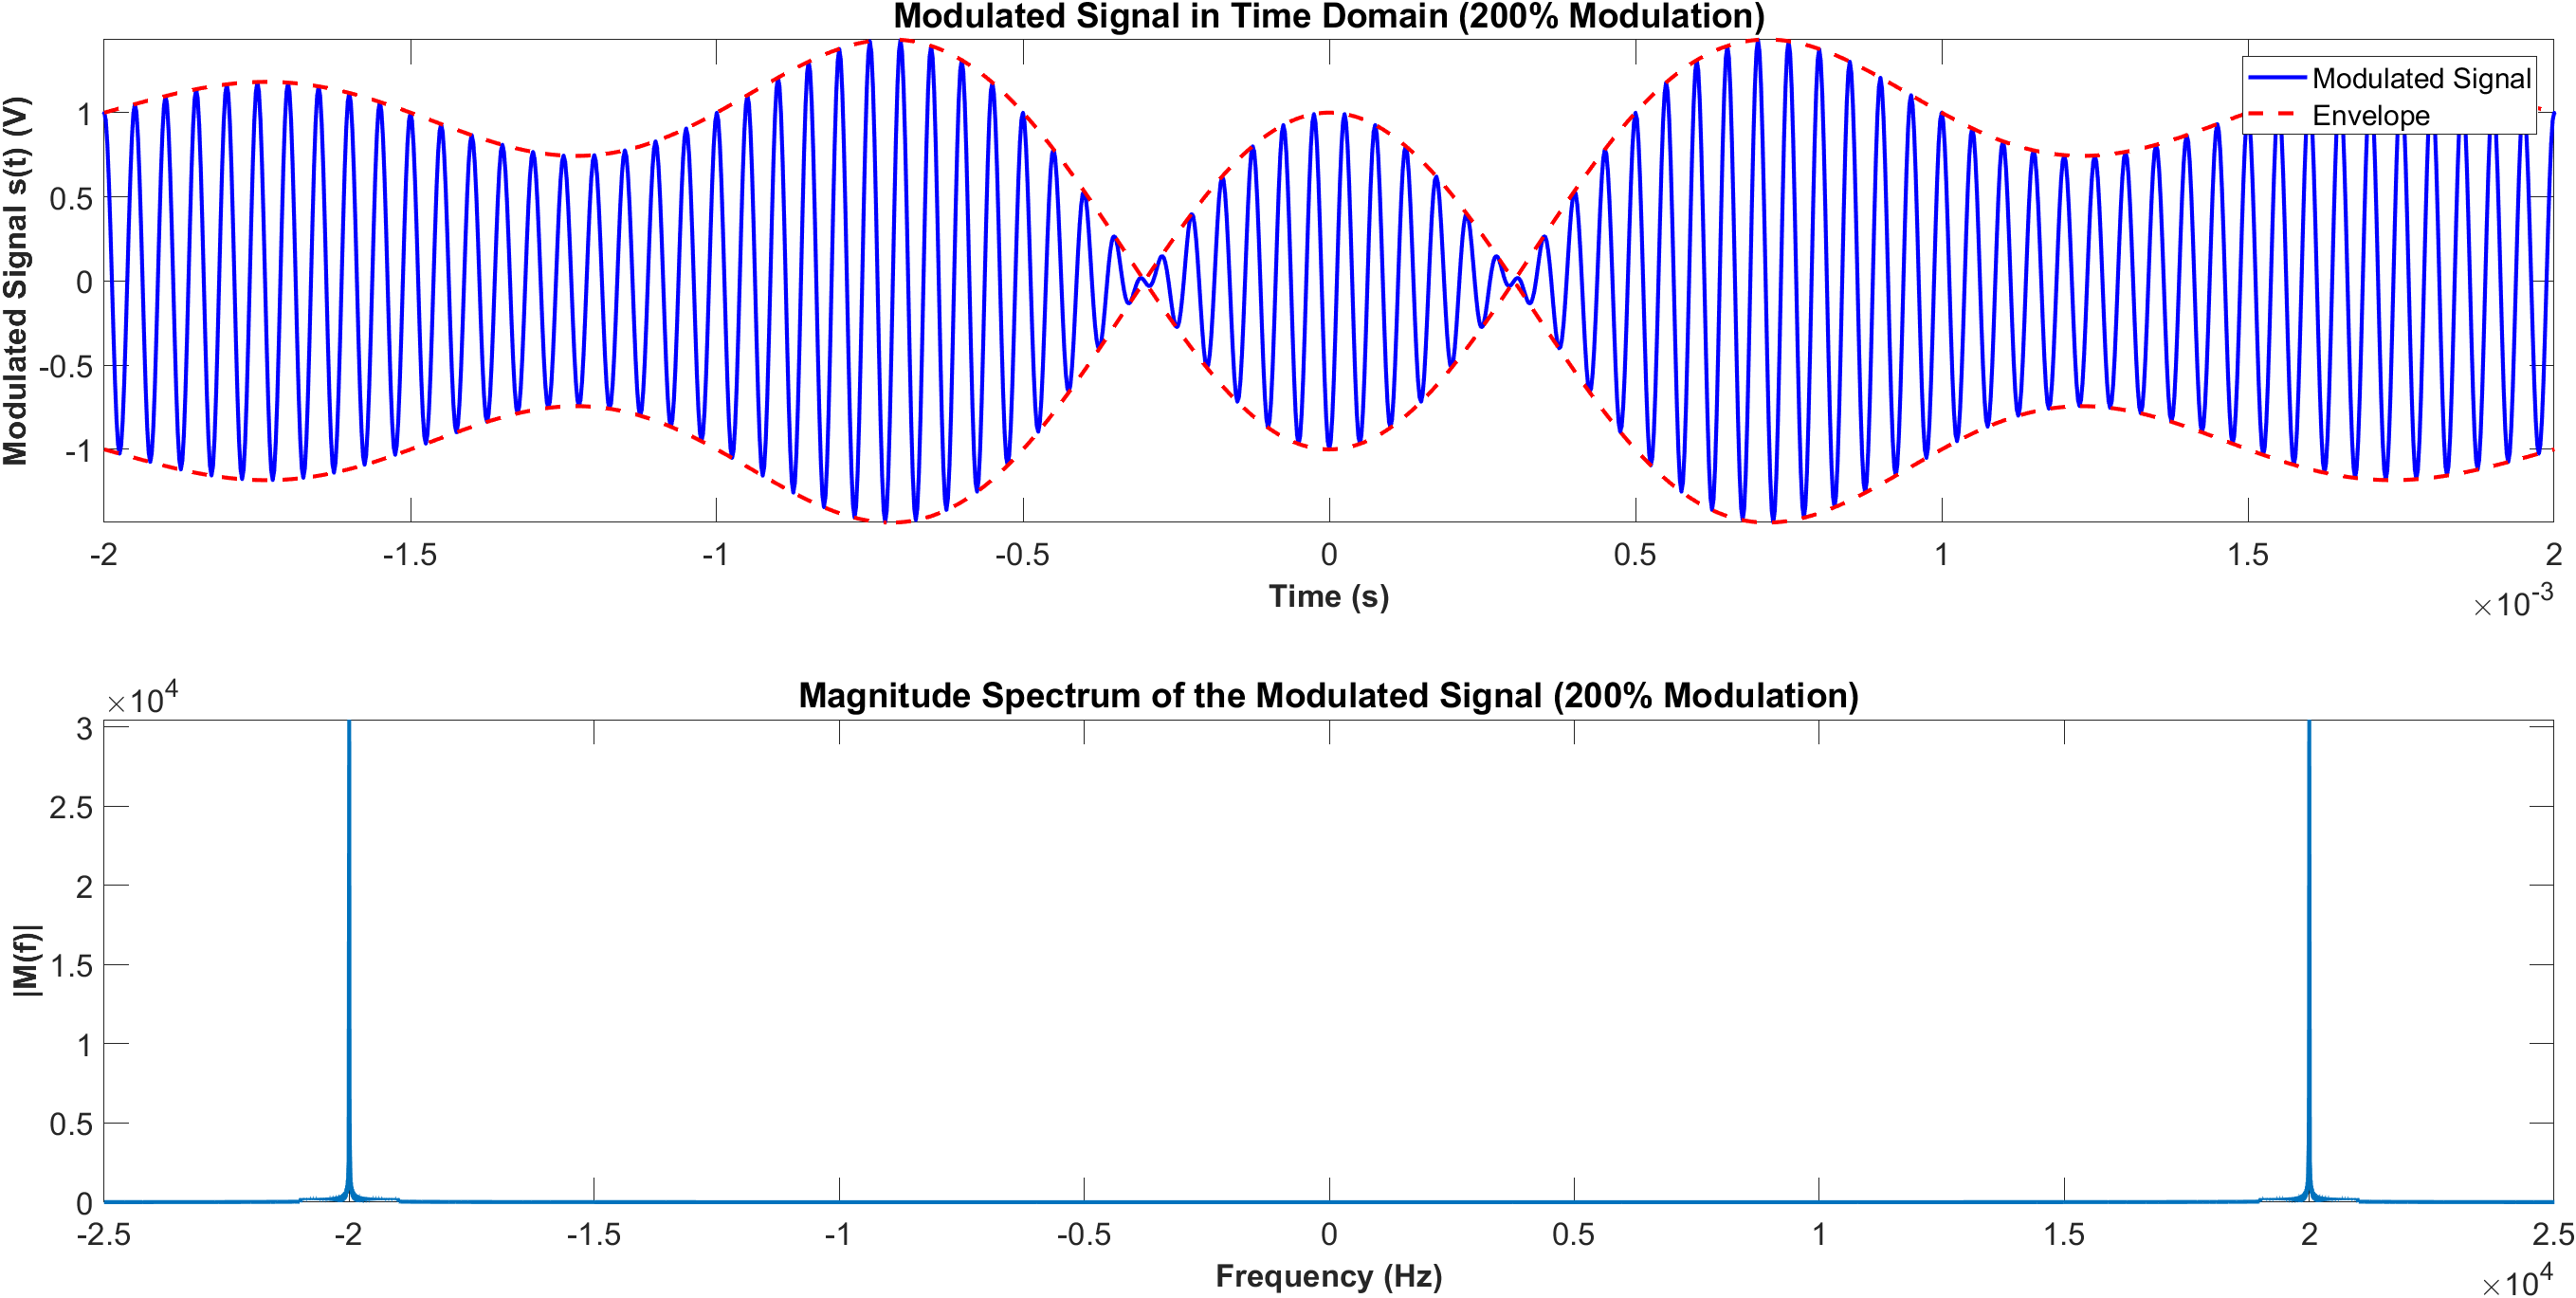
\includegraphics[width=\textwidth]{q3_mod}
    \caption{\label{fig:q3_mod}Modulated Signal with 200\% Modulation}
\end{figure}
\begin{figure}[h!]
    \centering
    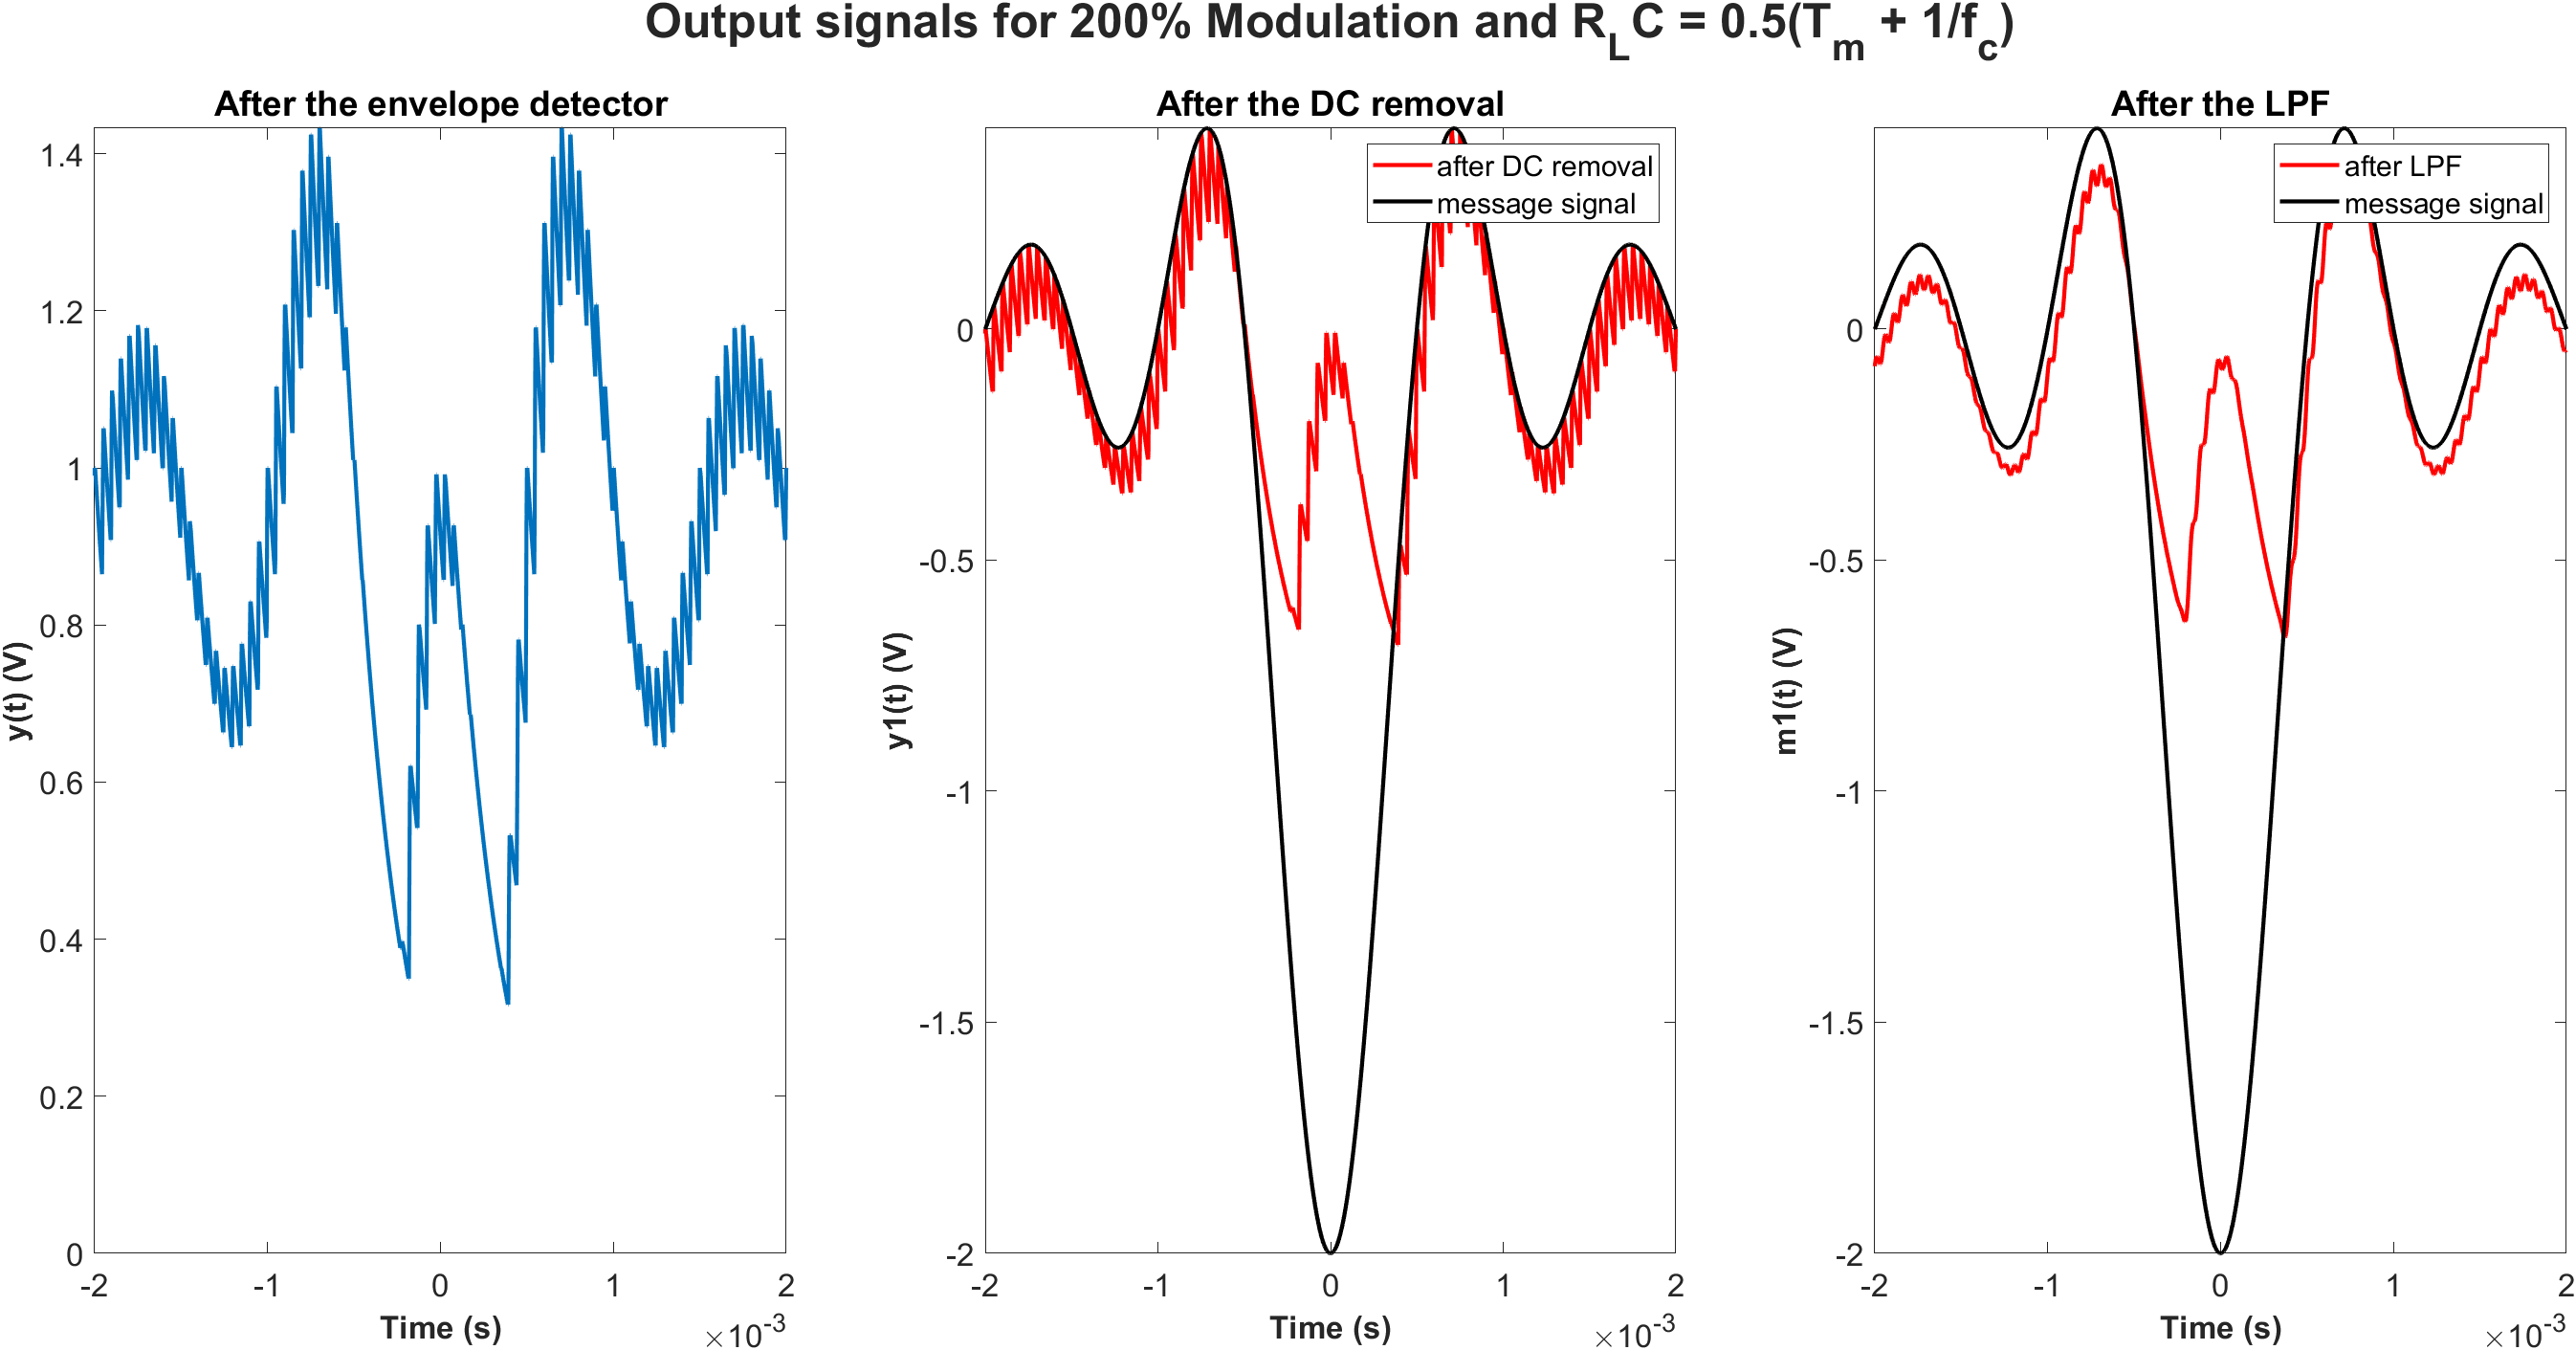
\includegraphics[width=\textwidth]{q3_demod}
    \caption{\label{fig:q3_demod}Demodulated Signal with 200\% Modulation}
\end{figure}


\end{document}